\documentclass[conference]{IEEEtran}

% Document properties
\title{On-chip order-exploiting routing table minimization for a multicast supercomputer network}
\author{%
  \IEEEauthorblockN{Andrew~Mundy, Jonathan~Heathcote and Jim~D.~Garside}
  \IEEEauthorblockA{School of Computer Science,\\
                    University of Manchester, UK}
}

% Prettier tables
\usepackage{booktabs}

% Pictures
\usepackage{graphicx}

% Pseudo-code
\usepackage{clrscode3e}

% Force float positions in some cases
\usepackage{float}

% Neaten the fixed-width font
\usepackage{sourcecodepro}
\newcommand{\mytt}[1]{\texttt{\footnotesize#1}}

\usepackage[binary-units]{siunitx}

%% Bibliographies
\usepackage[backend=bibtex, style=ieee, doi=false, url=false, mincitenames=1, maxcitenames=2, maxbibnames=7]{biblatex}
\bibliography{paper}

\begin{document}
  \maketitle

  \begin{abstract}
SpiNNaker is a many-core supercomputer, designed for the simulation of large neural-networks; cores communicate with multicast packets.
Routing within SpiNNaker is controlled by ternary content addressable memories (TCAM) of quite limited size.
However, not all neural-network applications will result in routing tables sufficiently small to fit in TCAM and some minimization is necessary.
In this paper we argue that existing minimization techniques either do not result in sufficiently minimized tables or cannot be implemented within the small code and memory footprint available to a SpiNNaker core.
To resolve these issues we present a new algorithm which exploits the ordered nature of the TCAM to achieve good compression of routing tables while meeting the code-space and memory constraints of the SpiNNaker platform.

  \end{abstract}

  \section{Introduction}

SpiNNaker~\parencite{Furber2014} is a purpose-built supercomputer intended to facilitate the simulation of large biological neural networks.
Software models are distributed across a network of processors which communicate by passing (short) messages.
Biological neurons in a brain typically have a `fanout' of the order of thousands and SpiNNaker's interconnection structure reflects this in that it supports multicasting network packets to an arbitrary set of destinations.

SpiNNaker comprises custom silicon where each chip has a single router capable of steering packets to or from the 18~on-chip processor cores and inter-chip links.
The inter-chip network is intended to be a triangularly connected 2D surface, nominally wrapped into a torus to provide greater aggregate bandwidth.
This can be drawn as a hexagonal mesh but is sometimes more conveniently pictured skewed into squares.
The six inter-chip links are typically labelled with compass points (fig. ???).

Routing these packets is done by Address Event Representation (AER)~\parencite{Boahen2000}; each packet contains a routing key which identifies its source and routers forward (and may duplicate) packets towards their destination(s).
SpiNNaker uses 32-bit routing keys which reflects the intended scale of the system: $\sim2^{16}$ SpiNNaker chips carry $\sim10^6$ processors or $\sim10^9 (\approx 2^{30})$ neurons, each of which must be uniquely identified.
Routers use a Ternary Content Addressable Memory (TCAM) to decide how to route incoming packets which bit-mask keys before looking for particular matches.
This means that each key bit can be matched with binary \mytt{0}, \mytt{1}, or \mytt{X} (`don't care').
In addition the TCAM is is prioritised such that only the first-found match will be returned and this allows `catch all' entries to be inserted near the bottom of the table.
Finally, if a key is not found in the table, the packet is `default routed' continuing in the direction it arrived (e.g. an unrecognised packet arriving via the East link is default routed out of the West link).

For a simplified example with 4-bit keys, given a routing table

\begin{table}[H]
  \centering
  \begin{tabular}{c l}
    \toprule
    Key-Mask & Route \\
    \midrule
    \texttt{0000} & \texttt{NE N}\\
    \texttt{X111} & \texttt{S}\\
    \texttt{1XXX} & \texttt{3 4}\\
    \bottomrule
  \end{tabular}
\end{table}

\noindent any packets with the keys \mytt{0111} or \mytt{1111} would match the second entry in the table and would be routed out of the South link.
Packets with the key \mytt{0000} would instead match only the first entry and would be routed out of both the North East and North links.
Other packets beginning with a \mytt{1} would match the last entry and would be routed to the indicated processing cores.
All other packets would be unrecognised by the router and are default routed in a straight line, e.g., a packet arriving on the South West link with the key \mytt{0011} would be routed out of the North East link.

The TCAM was chosen with an arbitrary size of 1024 entries, believed large enough for most applications although making entries quite precious.
Indeed, it is not always possible to avoid exceeding this limit on routing table size -- particularly for neural networks which feature large `fanin' or `fanout' routes.
As the largest SpiNNaker machine will consist of \num{57600} chips, and hence \num{57600} TCAM routing tables, it is desirable to exploit the massive parallelism of SpiNNaker to perform any minimisation of routing tables rather than to minimise tables externally before loading them to the machine. As we will show, this presents a challenge due to the limited on-chip memory available.

\section{Routing table minimization}

To indicate the importance of routing table minimization to SpiNNaker we constructed two benchmark networks.
In the first of these networks each processing core in a 144-chip system is connected to every other core in the system with a probability determined by the distance between the cores.
In our model the probability of there being a connection between two cores is given by $\frac{1}{2}\exp(-0.65d)$ where $d$ is the number of hops in the shortest path between the cores.
This benchmark models networks in which processing cores are strongly connected to their neighbours but are weakly connected to distant chips.

The second benchmark extends the first benchmark by adding a number of longer distance connections to the network and is based on the `centroid' model of \textcite{Navaridas2015}.
In this model a small number of cores are connected to a group of cores located at some distance across the machine.
Each core has a \SI{10}{\percent} chance of being connected to a single, distant, group of cores and a \SI{5}{\percent} chance of being connected to two distant groups.
\figurename~\ref{fig:experiment/setup} illustrates these two benchmarks and shows the probability of a single core being connected to other cores within the network.

\begin{figure}
  \centering
  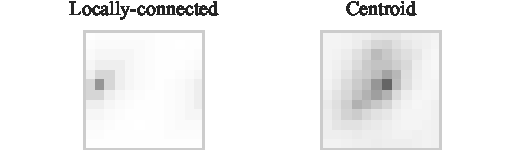
\includegraphics{experiments/experiments.pdf}
  \caption{Map of the probability of a single core being connected to cores on surrounding chips for the two benchmarks. Darker means higher probability.
           In the above centroid model the core is connected to two clusters of cores (toward the south west and north west).}
  \label{fig:experiment/setup}
\end{figure}

Once the connectivity of the benchmarks was determined, the Neighbour Exploring Routing (NER) algorithm~\parencite{Navaridas2015} was used to generate the routes taken by packets between cores.
This algorithm has been shown to effectively exploit `default routing' to reduce the size of routing tables; however, for both our benchmarks the resulting routing tables were still too large to fit in the number of entries available (see \figurename~\ref{fig:results/espresso_no_dc}).

\textcite{Liu2002} presented a method for using Espresso-II~\parencite{Brayton1984} to minimize routing tables for IP routing tables.
In this method a routing table is partitioned in subtables in which entries have equivalent routing destinations and prefix length.
Each subtable is minimized using Espresso to produce a functionally equivalent but smaller set of entries.
\figurename~\ref{fig:results/espresso_no_dc} shows the result of applying this technique to the routing tables from our benchmarks once entries which could be replaced by default routing were removed.
In the case of the `locally-connected' benchmark a combination of default routing and logic minimization is able to reduce the majority, but not all, of the 144 routing tables to fewer than 1024 entries.
In the more challenging centroid model this technique is unable to reduce any tables to fit within the TCAM constraint.

\begin{figure}
  \centering
  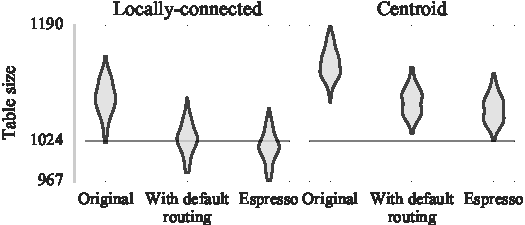
\includegraphics{experiments/results_no_dc}
  \caption{
    Distributions of routing table sizes for the locally-connected and centroid benchmarks.
    Neither default routing nor minimisation is sufficient to minimize the majority of tables in either benchmark sufficiently to fit within the 1024-entry limit required by SpiNNaker.}
  \label{fig:results/espresso_no_dc}
\end{figure}

In contrast to the unicast IP routing tables at which minimization is normally targeted SpiNNaker routing tables are multicast.
Consequently, there are two factors which may explain the poor compression ratios achieved by use of the above technique when applied to SpiNNaker routing tables.
Firstly, while the IP routing tables discussed by \textcite{Liu2002} have relatively few output ports, each SpiNNaker router has the equivalent of up to $2^{24} - 1$ unique routes -- consequently the number of entries with equivalent routes can be expected to be much smaller.
Secondly, whereas IP addresses are assigned such that very coarse routing decisions may be made from very few bits, multicasting potentially reduces the amount of mutual information between keys which describe similar routes since keys are related to route origins not destinations.

\subsection*{``Order-exploiting'' minimization}

Unlike IP routing tables, SpiNNaker routing tables can be expected to be largely static.
As such, logic minimization which does not preserve exact equivalence, but rather match a superset of the routing keys used, may be used to generate routing tables with far fewer entries.
For example, the first two entries in the table

  \begin{table}[H]
    \centering
    \begin{tabular}{c l l}
      \toprule
      Key-Mask & Route \\
      \midrule
      \texttt{0001} & \texttt{N} \\
      \texttt{0010} & \texttt{N} \\
      \texttt{1111} & \texttt{S} \\
      \bottomrule
    \end{tabular}
  \end{table}

\noindent may be combined into a new entry (\mytt{00XX}) which would match more keys than were matched by the original two entries.
In IP routing tables, which are considerably larger than those in SpiNNaker and are highly dynamic, this minimization would be avoided as it would (a) require the minimizer to inspect the entire table during minimization to avoid breaking the functionality of the table,
and (b) slow down the process of updating the table to deal with changed routes.
However, in the case of SpiNNaker -- and other systems with largely static routing tables and very tight constraints on entries -- this technique can allow for significant reductions in table size.

We extended the technique of \textcite{Liu2002} to investigate the effect of this style of minimization on our benchmark networks.
First, each routing table is split into subtables of entries with the same route.
Next the subtables are ordered in increasing order of the number of entries they contain; that is: smaller subtables are moved to the top of the routing table and larger ones toward the bottom.
Finally, the minimization procedure from Espresso is applied.
However, unlike the technique proposed by \textcite{Liu2002}, we provide Espresso with the set of all entries contained in lower subtables as the OFF-set.
Consequently each subtable is minimized such that the compressed subtable matches a superset of keys matched by the original subtable and may match any other keys \textit{not} matched in lower subtables.
The minimized table exploits TCAM ordering to ensure that a routing keys match the correct entries.
We term this use of table ordering to achieve greater compression of entries ``order-exploiting'' minimization.

\begin{figure}
  \centering
  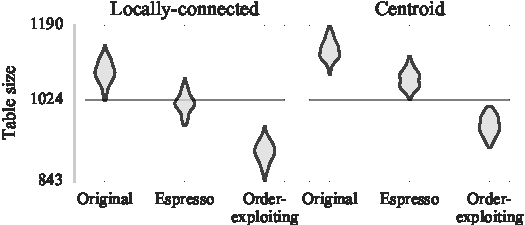
\includegraphics{experiments/results_with_dc}
  \caption{
    Distributions of routing table sizes for the locally-connected and centroid benchmarks for exact and order-exploiting use of Espresso.
  }
  \label{fig:results/espresso_with_dc}
\end{figure}

\figurename~\ref{fig:results/espresso_with_dc} shows that this new technique for reducing routing table size is sufficient to minimize all the routing tables in our benchmarks to fit within the 1024-entry size required by SpiNNaker.

\subsection*{On-chip logic minimization}

Espresso is capable of very rapidly minimizing routing tables of the scale shown in our benchmarks.
However, as projected SpiNNaker machines are expected to consist of nearly \num{60000} chips, and the same number of routing tables, the  compute time required to minimize all tables is likely to be significant.
Minimization on this scale is an `embarrassingly'-parallel problem, and the wall-clock time required to perform this task for SpiNNaker may be significantly reduced by performing the minimization directly on the chips to which the routing tables relate.

Processing cores in SpiNNaker have access to \SI{64}{\kibi\byte} of data tightly-coupled memory (DTCM) and \SI{32}{\kibi\byte} of instruction tightly-coupled memory (ITCM).
This places severe limitations on the programs which they may execute.
While we have shown that Espresso may be used to perform order-exploiting minimization for use with SpiNNaker, its memory usage and code size preclude its use on embedded systems~\parencite{Lysecky2003}.
In contrast, m-Trie minimization~\parencite{Ahmad2007} has been shown to be capable of effectively compressing IP routing tables while consuming very little memory (as low as \SI{16}{\kibi\byte}) but is not suitable for use when order-exploiting minimization is required.


\section{Ordered-Covering}

We present a novel algorithm called ``Ordered-Covering''~(OC) which is capable of performing order-exploiting routing table minimization within the small memory and code-space available on SpiNNaker.
Ordered Covering applies the following rules to ensure that the minimized routing table is behaviourally equivalent to the original:

  \begin{enumerate}[\IEEEsetlabelwidth{2)}]
    \item Routing tables are to be kept sorted in increasing order of the number of \mytt{X}s contained in their keys and masks, that is in increasing order of \textit{generality}.
      For example, an entry with the key-mask of \mytt{00XX} (\textit{generality} of 2) must be placed below any entries with fewer \mytt{X}s in their key-masks, e.g., below \mytt{0000} and \mytt{00X1} (generalities of 0 and 1 respectively).
      \begin{enumerate}[\IEEEsetlabelwidth{a)}]
        \item Additionally, new entries must be inserted below existing entries of equivalent generality.
              For example, if \mytt{XX00} were already present in the table the new entry \mytt{0XX1} must be inserted below it.
              This requirement is intended to reduce the cost of obeying the following two rules.
      \end{enumerate}
    \item Any merge may be made provided that it would not
      \begin{enumerate}[\IEEEsetlabelwidth{b)}]
        \item cause any entry in the merge to become \textit{covered} by an entry higher up the table.
              A merge that would be disallowed by this rule is shown in \figurename~\ref{fig:algorithm/rule2a_example}.
              This rule is referred to as the \textit{up-check} rule.
        \item cause any entry below the merge to become covered (see \figurename~\ref{fig:algorithm/rule2b_example}).
              This rule is referred to as the \textit{down-check} rule.
      \end{enumerate}
  \end{enumerate}

  \begin{figure}
    \centering
    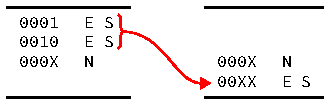
\includegraphics{figures/rule2a_example}
    \caption{
      Example of a merge which does not obey rule~(2a), the \textit{up-check}.
      Before the merge a packet with key \mytt{0001} would have been routed to \mytt{E~S}; after the merge the same packet would be routed to \mytt{N} instead.
      This is because the merge has resulted in the correct entry being moved below an entry which \textit{covers} it.
    }
    \label{fig:algorithm/rule2a_example}
  \end{figure}

  \begin{figure}
    \centering
    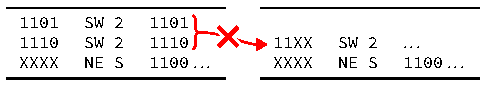
\includegraphics{figures/rule2b_example}
    \caption{
      Example of a merge which does not obey rule~(2b), the \textit{down-check}.
      Before the merge a packet with key \mytt{1100} would have been routed to \mytt{NE~S}; after the merge the same packet would be routed to \mytt{SW 2} instead.
      This is because the merge has resulted in the insertion of a new entry which \textit{covers} an existing entry.
    }
    \label{fig:algorithm/rule2b_example}
  \end{figure}

  These rules may be transformed into a simple, greedy, algorithm to minimize a routing table:

  \begin{codebox}
    \Procname{$\proc{Minimize}(\id{table}, \id{target})$}
    \li \While $\attrib{table}{length} >  \id{target}$
    \li \Do $\id{merge} \gets \proc{Get-Largest-Merge}(\id{table})$
    \li     \If $\attrib{merge}{isEmpty}$
    \li     \Then \kw{break} \End
    \li     $\id{table} \gets \proc{Apply-Merge}(\id{table}, \id{merge})$
        \End
    \li \Return $\id{table}$
  \end{codebox}

  \noindent Where:
  \begin{itemize}
    \item $\id{table}$ is a routing table that is sorted according to rule~(1)
    \item $\proc{Get-Largest-Merge}$ is a function which returns a (possibly empty) set of routing table entries which may be merged without breaking rule~(2)
    \item $\proc{Apply-Merge}$ applies a merge to a routing table using rule~(1) to determine where the new entry should be inserted
  \end{itemize}

  It should be noted that the algorithm terminates when $\attrib{table}{length} \le \id{target}$.
  This can save a large amount of time in comparison to fully minimizing the table.

  Merge candidates may be made by any means, in our implementation we attempt to merge all entries in the table with the same routing direction.
  Initially $\proc{Get-Largest-Merge}$ should immediately reject any merge candidate which breaks either rule~(2a)~or~(2b).
  However, this will lead to very poor minimization.
  To improve performance methods are required which modify potential merges such that they obey both rules.

  \subsection{Resolving the up-check}

  To ensure that a merge does not break rule (2a) we inspect every entry in the merge.
  If between the position where the entry resulting from the merge would be inserted and the current position of the entry there is an entry which matches the entry in question then that entry must be removed from merge.

  For example, consider the table:

  \begin{figure}[H]
    \centering
    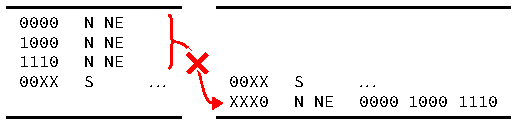
\includegraphics{figures/upcheck_resolve_example_1}
  \end{figure}

  \noindent Initially we consider merging the first three entries.
  Doing so, however, would involve moving the entry for \mytt{0000} below \mytt{00XX}.
  As \mytt{0000} intersects with \mytt{00XX} it must be removed from the merge, resulting in:

  \begin{figure}[H]
    \centering
    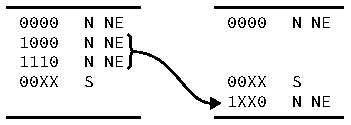
\includegraphics{figures/upcheck_resolve_example_2}
  \end{figure}

  \noindent which is a valid merge.

  \subsection{Resolving the down-check}
  
  Rule~(2b) disallows any merges which would create a new entry that would cover any entries below the point where it would be inserted.
  However, if routing table entries are annotated with the keys (expressed as key-masks) that they are expected to match then rule~(2b) can be re-expressed as:

  \begin{quote}
    Any merge may be made provided that it would not cause any key which is expected to be matched by an entry below the merge to become covered.
  \end{quote}

  \figurename~\ref{fig:algorithm/rule2b'_example} shows an example of a merge which would previously have been disallowed by rule~(2b) but would be valid given extra information and this revision to rule~(2b).

  \begin{figure}[!b]
    \centering
    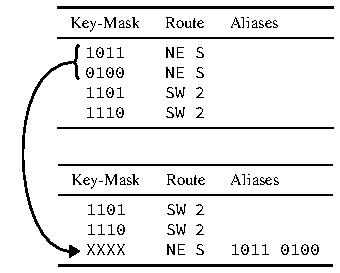
\includegraphics{figures/aliases_example}
    \caption{
      Example of a merge which does not obey rule~(2b), the \textit{down-check}, but is valid if extra information about which keys are expected to reach which entries is provided.
      While the merge would result in a packet with key \mytt{1100} being routed differently, \textit{no such packet is expected to reach the bottom routing table entry} and neither of the keys that are expected (\mytt{1011} and \mytt{0100}) will match the entry inserted by the merge (\mytt{11XX}).
    }
    \label{fig:algorithm/rule2b'_example}
  \end{figure}

  Consider the table:

  \begin{table}[H]
    \centering
    \begin{tabular}{c l l}
      \toprule
      Key-Mask & Route & Aliases \\
      \midrule
      \textbf{\texttt{1100}} & \texttt{N} \\
      \textbf{\texttt{1101}} & \texttt{N} \\
      \textbf{\texttt{111X}} & \texttt{N} \\
      \texttt{XXXX} & \texttt{4} & \texttt{0100}, \texttt{1011}, \texttt{1110} \\
      \bottomrule
    \end{tabular}
  \end{table}

  The first three entries cannot be merged because the merged entry (\mytt{11XX}) would be inserted above the bottom entry and would prevent packets with the key \mytt{1110} from being routed correctly.

  To proceed we attempt to find bits which are \mytt{X}s in the merged entry but are not \mytt{X}s in the covered entry.
  In this example this is the two rightmost bits, \mytt{11\underline{XX}} and \mytt{11\underline{10}} for the merged and covered entries respectively.
  To resolve the covering we attempt to remove entries from the merge such that one of the \mytt{X}s we just identified becomes the opposite of the covered value in the same position.
  In this example, we look to remove entries from the merge such that the merged entry is either \mytt{11\underline{X1}} or \mytt{11\underline{0X}}.

  To `set' the entry resulting from the merge to \mytt{11X\underline{1}} we need to remove from the merge any entries with an \mytt{X} or \mytt{0} in the rightmost bit.
  In this case removing the entries with the key-mask \mytt{110\underline{0}} and \mytt{111\underline{X}} is sufficient.
  Alternatively, to set the entry resulting from the merge to \mytt{11\underline{0}X} we need to remove from the merge any entries with an \mytt{X} or \mytt{1} in the second rightmost bit.
  This would entail removing the entry with the key-mask \mytt{111X} from the merge.

  As we want to merge as many entries as possible we greedily select to remove the fewest number of entries from the merge.
  The new merge candidate is then:

  \begin{table}[H]
    \centering
    \begin{tabular}{c l l}
      \toprule
      \textbf{\texttt{1100}} & \texttt{N} \\
      \textbf{\texttt{1101}} & \texttt{N} \\
      \texttt{111X} & \texttt{N} \\
      \texttt{XXXX} & \texttt{4} & \texttt{0100}, \texttt{1011}, \texttt{1110} \\
      \bottomrule
    \end{tabular}
  \end{table}

  Which would result in the new entry \mytt{110X} being inserted between \mytt{111X} and \mytt{XXXX}.
  This merge does not result in any of its constituent entries becoming covered (rule 2a) and does not prevent any of the keys expected by lower entries from reaching them (rule 2b) and so the merge may proceed.

  \section{Results}

  TODO:
  \begin{itemize}
    \item Andrew has some memory results, but basically a 2048-entry table will fit in memory fine assuming the alias table is implemented sanely.
    \item Algorithm is complex but effective; code fits in 13KiB
    \item Something to do with timing (very quick results to grab)
    \item Jonathan? Something about using multiple cores to minimise as far as necessary.
    \item Andrew: resurrect circular convolution model?
  \end{itemize}
  
    \subsection{Hedging}
    
       Each SpiNNaker chip has 18 processor cores and one routing table enabling parallel table minimisation approaches.
       It is possible to execute several table minimisation algorithms simultaneously, terminating as soon as any algorithm produces a table which fits.
       This approach may be valuable in cases where default routing is sufficient since these routes are very cheap to compute.

\begin{figure}
  \centering
  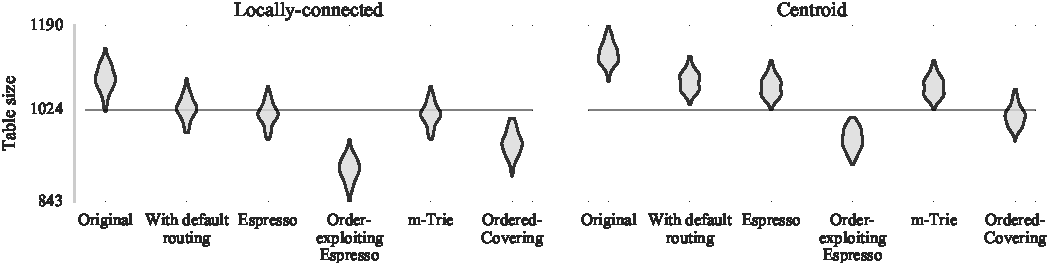
\includegraphics{experiments/results_esp_and_oc}
\end{figure}

  \section{Conclusion}

\printbibliography
\end{document}
